\documentclass[1p]{elsarticle_modified}
%\bibliographystyle{elsarticle-num}

%\usepackage[colorlinks]{hyperref}
%\usepackage{abbrmath_seonhwa} %\Abb, \Ascr, \Acal ,\Abf, \Afrak
\usepackage{amsfonts}
\usepackage{amssymb}
\usepackage{amsmath}
\usepackage{amsthm}
\usepackage{scalefnt}
\usepackage{amsbsy}
\usepackage{kotex}
\usepackage{caption}
\usepackage{subfig}
\usepackage{color}
\usepackage{graphicx}
\usepackage{xcolor} %% white, black, red, green, blue, cyan, magenta, yellow
\usepackage{float}
\usepackage{setspace}
\usepackage{hyperref}

\usepackage{tikz}
\usetikzlibrary{arrows}

\usepackage{multirow}
\usepackage{array} % fixed length table
\usepackage{hhline}

%%%%%%%%%%%%%%%%%%%%%
\makeatletter
\renewcommand*\env@matrix[1][\arraystretch]{%
	\edef\arraystretch{#1}%
	\hskip -\arraycolsep
	\let\@ifnextchar\new@ifnextchar
	\array{*\c@MaxMatrixCols c}}
\makeatother %https://tex.stackexchange.com/questions/14071/how-can-i-increase-the-line-spacing-in-a-matrix
%%%%%%%%%%%%%%%

\usepackage[normalem]{ulem}

\newcommand{\msout}[1]{\ifmmode\text{\sout{\ensuremath{#1}}}\else\sout{#1}\fi}
%SOURCE: \msout is \stkout macro in https://tex.stackexchange.com/questions/20609/strikeout-in-math-mode

\newcommand{\cancel}[1]{
	\ifmmode
	{\color{red}\msout{#1}}
	\else
	{\color{red}\sout{#1}}
	\fi
}

\newcommand{\add}[1]{
	{\color{blue}\uwave{#1}}
}

\newcommand{\replace}[2]{
	\ifmmode
	{\color{red}\msout{#1}}{\color{blue}\uwave{#2}}
	\else
	{\color{red}\sout{#1}}{\color{blue}\uwave{#2}}
	\fi
}

\newcommand{\Sol}{\mathcal{S}} %segment
\newcommand{\D}{D} %diagram
\newcommand{\A}{\mathcal{A}} %arc


%%%%%%%%%%%%%%%%%%%%%%%%%%%%%5 test

\def\sl{\operatorname{\textup{SL}}(2,\Cbb)}
\def\psl{\operatorname{\textup{PSL}}(2,\Cbb)}
\def\quan{\mkern 1mu \triangleright \mkern 1mu}

\theoremstyle{definition}
\newtheorem{thm}{Theorem}[section]
\newtheorem{prop}[thm]{Proposition}
\newtheorem{lem}[thm]{Lemma}
\newtheorem{ques}[thm]{Question}
\newtheorem{cor}[thm]{Corollary}
\newtheorem{defn}[thm]{Definition}
\newtheorem{exam}[thm]{Example}
\newtheorem{rmk}[thm]{Remark}
\newtheorem{alg}[thm]{Algorithm}

\newcommand{\I}{\sqrt{-1}}
\begin{document}

%\begin{frontmatter}
%
%\title{Boundary parabolic representations of knots up to 8 crossings}
%
%%% Group authors per affiliation:
%\author{Yunhi Cho} 
%\address{Department of Mathematics, University of Seoul, Seoul, Korea}
%\ead{yhcho@uos.ac.kr}
%
%
%\author{Seonhwa Kim} %\fnref{s_kim}}
%\address{Center for Geometry and Physics, Institute for Basic Science, Pohang, 37673, Korea}
%\ead{ryeona17@ibs.re.kr}
%
%\author{Hyuk Kim}
%\address{Department of Mathematical Sciences, Seoul National University, Seoul 08826, Korea}
%\ead{hyukkim@snu.ac.kr}
%
%\author{Seokbeom Yoon}
%\address{Department of Mathematical Sciences, Seoul National University, Seoul, 08826,  Korea}
%\ead{sbyoon15@snu.ac.kr}
%
%\begin{abstract}
%We find all boundary parabolic representation of knots up to 8 crossings.
%
%\end{abstract}
%\begin{keyword}
%    \MSC[2010] 57M25 
%\end{keyword}
%
%\end{frontmatter}

%\linenumbers
%\tableofcontents
%
\newcommand\colored[1]{\textcolor{white}{\rule[-0.35ex]{0.8em}{1.4ex}}\kern-0.8em\color{red} #1}%
%\newcommand\colored[1]{\textcolor{white}{ #1}\kern-2.17ex	\textcolor{white}{ #1}\kern-1.81ex	\textcolor{white}{ #1}\kern-2.15ex\color{red}#1	}

{\Large $\underline{12a_{0718}~(K12a_{0718})}$}

\setlength{\tabcolsep}{10pt}
\renewcommand{\arraystretch}{1.6}
\vspace{1cm}\begin{tabular}{m{100pt}>{\centering\arraybackslash}m{274pt}}
\multirow{5}{120pt}{
	\centering
	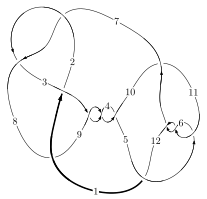
\includegraphics[width=112pt]{../../../GIT/diagram.site/Diagrams/png/1519_12a_0718.png}\\
\ \ \ A knot diagram\footnotemark}&
\allowdisplaybreaks
\textbf{Linearized knot diagam} \\
\cline{2-2}
 &
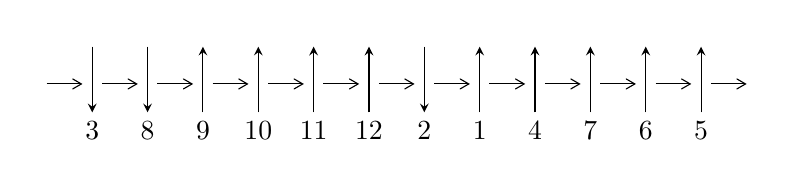
\begin{tikzpicture}[x=20pt, y=17pt]
	% nodes
	\node (C0) at (0, 0) {};
	\node (C1) at (1, 0) {};
	\node (C1U) at (1, +1) {};
	\node (C1D) at (1, -1) {3};

	\node (C2) at (2, 0) {};
	\node (C2U) at (2, +1) {};
	\node (C2D) at (2, -1) {8};

	\node (C3) at (3, 0) {};
	\node (C3U) at (3, +1) {};
	\node (C3D) at (3, -1) {9};

	\node (C4) at (4, 0) {};
	\node (C4U) at (4, +1) {};
	\node (C4D) at (4, -1) {10};

	\node (C5) at (5, 0) {};
	\node (C5U) at (5, +1) {};
	\node (C5D) at (5, -1) {11};

	\node (C6) at (6, 0) {};
	\node (C6U) at (6, +1) {};
	\node (C6D) at (6, -1) {12};

	\node (C7) at (7, 0) {};
	\node (C7U) at (7, +1) {};
	\node (C7D) at (7, -1) {2};

	\node (C8) at (8, 0) {};
	\node (C8U) at (8, +1) {};
	\node (C8D) at (8, -1) {1};

	\node (C9) at (9, 0) {};
	\node (C9U) at (9, +1) {};
	\node (C9D) at (9, -1) {4};

	\node (C10) at (10, 0) {};
	\node (C10U) at (10, +1) {};
	\node (C10D) at (10, -1) {7};

	\node (C11) at (11, 0) {};
	\node (C11U) at (11, +1) {};
	\node (C11D) at (11, -1) {6};

	\node (C12) at (12, 0) {};
	\node (C12U) at (12, +1) {};
	\node (C12D) at (12, -1) {5};
	\node (C13) at (13, 0) {};

	% arrows
	\draw[->,>={angle 60}]
	(C0) edge (C1) (C1) edge (C2) (C2) edge (C3) (C3) edge (C4) (C4) edge (C5) (C5) edge (C6) (C6) edge (C7) (C7) edge (C8) (C8) edge (C9) (C9) edge (C10) (C10) edge (C11) (C11) edge (C12) (C12) edge (C13) ;	\draw[->,>=stealth]
	(C1U) edge (C1D) (C2U) edge (C2D) (C3D) edge (C3U) (C4D) edge (C4U) (C5D) edge (C5U) (C6D) edge (C6U) (C7U) edge (C7D) (C8D) edge (C8U) (C9D) edge (C9U) (C10D) edge (C10U) (C11D) edge (C11U) (C12D) edge (C12U) ;
	\end{tikzpicture} \\
\hhline{~~} \\& 
\textbf{Solving Sequence} \\ \cline{2-2} 
 &
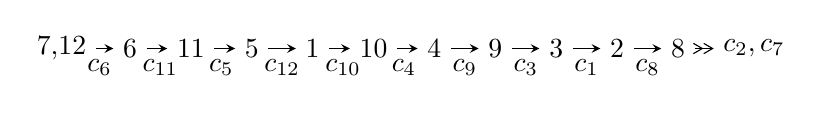
\begin{tikzpicture}[x=22pt, y=7pt]
	% node
	\node (A0) at (-1/8, 0) {7,12};
	\node (A1) at (1, 0) {6};
	\node (A2) at (2, 0) {11};
	\node (A3) at (3, 0) {5};
	\node (A4) at (4, 0) {1};
	\node (A5) at (5, 0) {10};
	\node (A6) at (6, 0) {4};
	\node (A7) at (7, 0) {9};
	\node (A8) at (8, 0) {3};
	\node (A9) at (9, 0) {2};
	\node (A10) at (10, 0) {8};
	\node (C1) at (1/2, -1) {$c_{6}$};
	\node (C2) at (3/2, -1) {$c_{11}$};
	\node (C3) at (5/2, -1) {$c_{5}$};
	\node (C4) at (7/2, -1) {$c_{12}$};
	\node (C5) at (9/2, -1) {$c_{10}$};
	\node (C6) at (11/2, -1) {$c_{4}$};
	\node (C7) at (13/2, -1) {$c_{9}$};
	\node (C8) at (15/2, -1) {$c_{3}$};
	\node (C9) at (17/2, -1) {$c_{1}$};
	\node (C10) at (19/2, -1) {$c_{8}$};
	\node (A11) at (45/4, 0) {$c_{2},c_{7}$};

	% edge
	\draw[->,>=stealth]	
	(A0) edge (A1) (A1) edge (A2) (A2) edge (A3) (A3) edge (A4) (A4) edge (A5) (A5) edge (A6) (A6) edge (A7) (A7) edge (A8) (A8) edge (A9) (A9) edge (A10) ;
	\draw[->>,>={angle 60}]	
	(A10) edge (A11);
\end{tikzpicture} \\ 

\end{tabular} \\

\footnotetext{
The image of knot diagram is generated by the software ``\textbf{Draw programme}" developed by Andrew Bartholomew(\url{http://www.layer8.co.uk/maths/draw/index.htm\#Running-draw}), where we modified some parts for our purpose(\url{https://github.com/CATsTAILs/LinksPainter}).
}\phantom \\ \newline 
\centering \textbf{Ideals for irreducible components\footnotemark of $X_{\text{par}}$} 
 
\begin{align*}
I^u_{1}&=\langle 
u^{69}-2 u^{68}+\cdots+2 u^2-1\rangle \\
I^u_{2}&=\langle 
u+1\rangle \\
\\
\end{align*}
\raggedright * 2 irreducible components of $\dim_{\mathbb{C}}=0$, with total 70 representations.\\
\footnotetext{All coefficients of polynomials are rational numbers. But the coefficients are sometimes approximated in decimal forms when there is not enough margin.}
\newpage
\renewcommand{\arraystretch}{1}
\centering \section*{I. $I^u_{1}= \langle u^{69}-2 u^{68}+\cdots+2 u^2-1 \rangle$}
\flushleft \textbf{(i) Arc colorings}\\
\begin{tabular}{m{7pt} m{180pt} m{7pt} m{180pt} }
\flushright $a_{7}=$&$\begin{pmatrix}1\\0\end{pmatrix}$ \\
\flushright $a_{12}=$&$\begin{pmatrix}0\\u\end{pmatrix}$ \\
\flushright $a_{6}=$&$\begin{pmatrix}1\\u^2\end{pmatrix}$ \\
\flushright $a_{11}=$&$\begin{pmatrix}- u\\- u^3+u\end{pmatrix}$ \\
\flushright $a_{5}=$&$\begin{pmatrix}- u^2+1\\- u^4+2 u^2\end{pmatrix}$ \\
\flushright $a_{1}=$&$\begin{pmatrix}u^5-2 u^3+u\\u^7-3 u^5+2 u^3+u\end{pmatrix}$ \\
\flushright $a_{10}=$&$\begin{pmatrix}u^3-2 u\\- u^3+u\end{pmatrix}$ \\
\flushright $a_{4}=$&$\begin{pmatrix}u^{10}-5 u^8+8 u^6-3 u^4-3 u^2+1\\- u^{10}+4 u^8-5 u^6+3 u^2\end{pmatrix}$ \\
\flushright $a_{9}=$&$\begin{pmatrix}- u^{17}+8 u^{15}-25 u^{13}+36 u^{11}-17 u^9-12 u^7+12 u^5+2 u^3-3 u\\u^{17}-7 u^{15}+19 u^{13}-22 u^{11}+3 u^9+14 u^7-6 u^5-4 u^3+u\end{pmatrix}$ \\
\flushright $a_{3}=$&$\begin{pmatrix}- u^{24}+11 u^{22}+\cdots-6 u^2+1\\u^{24}-10 u^{22}+\cdots-2 u^4+4 u^2\end{pmatrix}$ \\
\flushright $a_{2}=$&$\begin{pmatrix}- u^{55}+24 u^{53}+\cdots-28 u^5+12 u^3\\u^{55}-23 u^{53}+\cdots-2 u^3+u\end{pmatrix}$ \\
\flushright $a_{8}=$&$\begin{pmatrix}- u^{29}+12 u^{27}+\cdots-2 u^3-3 u\\- u^{31}+13 u^{29}+\cdots-8 u^3+u\end{pmatrix}$\\&\end{tabular}
\flushleft \textbf{(ii) Obstruction class $= -1$}\\~\\
\flushleft \textbf{(iii) Cusp Shapes $= 4 u^{68}-116 u^{66}+\cdots-8 u+10$}\\~\\
\newpage\renewcommand{\arraystretch}{1}
\flushleft \textbf{(iv) u-Polynomials at the component}\newline \\
\begin{tabular}{m{50pt}|m{274pt}}
Crossings & \hspace{64pt}u-Polynomials at each crossing \\
\hline $$\begin{aligned}c_{1}\end{aligned}$$&$\begin{aligned}
&u^{69}+30 u^{68}+\cdots+4 u+1
\end{aligned}$\\
\hline $$\begin{aligned}c_{2},c_{7}\end{aligned}$$&$\begin{aligned}
&u^{69}+2 u^{68}+\cdots-2 u^2+1
\end{aligned}$\\
\hline $$\begin{aligned}c_{3},c_{4},c_{9}\end{aligned}$$&$\begin{aligned}
&u^{69}-35 u^{67}+\cdots+16 u+1
\end{aligned}$\\
\hline $$\begin{aligned}c_{5},c_{6},c_{11}\end{aligned}$$&$\begin{aligned}
&u^{69}+2 u^{68}+\cdots-2 u^2+1
\end{aligned}$\\
\hline $$\begin{aligned}c_{8}\end{aligned}$$&$\begin{aligned}
&u^{69}+3 u^{68}+\cdots-8 u-1
\end{aligned}$\\
\hline $$\begin{aligned}c_{10},c_{12}\end{aligned}$$&$\begin{aligned}
&u^{69}-3 u^{68}+\cdots+4 u-1
\end{aligned}$\\
\hline
\end{tabular}\\~\\
\newpage\renewcommand{\arraystretch}{1}
\flushleft \textbf{(v) Riley Polynomials at the component}\newline \\
\begin{tabular}{m{50pt}|m{274pt}}
Crossings & \hspace{64pt}Riley Polynomials at each crossing \\
\hline $$\begin{aligned}c_{1}\end{aligned}$$&$\begin{aligned}
&y^{69}+18 y^{68}+\cdots-28 y-1
\end{aligned}$\\
\hline $$\begin{aligned}c_{2},c_{7}\end{aligned}$$&$\begin{aligned}
&y^{69}-30 y^{68}+\cdots+4 y-1
\end{aligned}$\\
\hline $$\begin{aligned}c_{3},c_{4},c_{9}\end{aligned}$$&$\begin{aligned}
&y^{69}-70 y^{68}+\cdots+100 y-1
\end{aligned}$\\
\hline $$\begin{aligned}c_{5},c_{6},c_{11}\end{aligned}$$&$\begin{aligned}
&y^{69}-58 y^{68}+\cdots+4 y-1
\end{aligned}$\\
\hline $$\begin{aligned}c_{8}\end{aligned}$$&$\begin{aligned}
&y^{69}-3 y^{68}+\cdots+4 y-1
\end{aligned}$\\
\hline $$\begin{aligned}c_{10},c_{12}\end{aligned}$$&$\begin{aligned}
&y^{69}+33 y^{68}+\cdots-12 y-1
\end{aligned}$\\
\hline
\end{tabular}\\~\\
\newpage\flushleft \textbf{(vi) Complex Volumes and Cusp Shapes}
$$\begin{array}{c|c|c}  
\text{Solutions to }I^u_{1}& \I (\text{vol} + \sqrt{-1}CS) & \text{Cusp shape}\\
 \hline 
\begin{aligned}
u &= -0.957601 + 0.300766 I\end{aligned}
 & \phantom{-}5.05918 + 6.89076 I & \phantom{-}6.00000 - 4.16482 I \\ \hline\begin{aligned}
u &= -0.957601 - 0.300766 I\end{aligned}
 & \phantom{-}5.05918 - 6.89076 I & \phantom{-}6.00000 + 4.16482 I \\ \hline\begin{aligned}
u &= -0.970924 + 0.140812 I\end{aligned}
 & \phantom{-}1.64199 + 0.00698 I & \phantom{-}6.00000 + 0. I\phantom{ +0.000000I} \\ \hline\begin{aligned}
u &= -0.970924 - 0.140812 I\end{aligned}
 & \phantom{-}1.64199 - 0.00698 I & \phantom{-}6.00000 + 0. I\phantom{ +0.000000I} \\ \hline\begin{aligned}
u &= \phantom{-}0.933707 + 0.288136 I\end{aligned}
 & \phantom{-}6.89512 - 1.63728 I & \phantom{-}11.63888 + 0. I\phantom{ +0.000000I} \\ \hline\begin{aligned}
u &= \phantom{-}0.933707 - 0.288136 I\end{aligned}
 & \phantom{-}6.89512 + 1.63728 I & \phantom{-}11.63888 + 0. I\phantom{ +0.000000I} \\ \hline\begin{aligned}
u &= \phantom{-}0.857602 + 0.279930 I\end{aligned}
 & \phantom{-}7.01858 + 1.34841 I & \phantom{-}12.02587 - 1.24080 I \\ \hline\begin{aligned}
u &= \phantom{-}0.857602 - 0.279930 I\end{aligned}
 & \phantom{-}7.01858 - 1.34841 I & \phantom{-}12.02587 + 1.24080 I \\ \hline\begin{aligned}
u &= -0.825401 + 0.288872 I\end{aligned}
 & \phantom{-}5.28751 - 6.59810 I & \phantom{-}9.41471 + 6.14577 I \\ \hline\begin{aligned}
u &= -0.825401 - 0.288872 I\end{aligned}
 & \phantom{-}5.28751 + 6.59810 I & \phantom{-}9.41471 - 6.14577 I \\ \hline\begin{aligned}
u &= -0.189683 + 0.774659 I\end{aligned}
 & \phantom{-}2.65904 - 10.93250 I & \phantom{-}5.56084 + 8.27245 I \\ \hline\begin{aligned}
u &= -0.189683 - 0.774659 I\end{aligned}
 & \phantom{-}2.65904 + 10.93250 I & \phantom{-}5.56084 - 8.27245 I \\ \hline\begin{aligned}
u &= \phantom{-}0.193338 + 0.767498 I\end{aligned}
 & \phantom{-}4.55534 + 5.62792 I & \phantom{-}8.38609 - 3.88248 I \\ \hline\begin{aligned}
u &= \phantom{-}0.193338 - 0.767498 I\end{aligned}
 & \phantom{-}4.55534 - 5.62792 I & \phantom{-}8.38609 + 3.88248 I \\ \hline\begin{aligned}
u &= \phantom{-}1.184060 + 0.293256 I\end{aligned}
 & -1.37585 - 2.62316 I & \phantom{-0.000000 } 0 \\ \hline\begin{aligned}
u &= \phantom{-}1.184060 - 0.293256 I\end{aligned}
 & -1.37585 + 2.62316 I & \phantom{-0.000000 } 0 \\ \hline\begin{aligned}
u &= \phantom{-}0.205061 + 0.747895 I\end{aligned}
 & \phantom{-}4.87077 + 2.53274 I & \phantom{-}8.88434 - 3.60320 I \\ \hline\begin{aligned}
u &= \phantom{-}0.205061 - 0.747895 I\end{aligned}
 & \phantom{-}4.87077 - 2.53274 I & \phantom{-}8.88434 + 3.60320 I \\ \hline\begin{aligned}
u &= -0.177328 + 0.752440 I\end{aligned}
 & -0.80018 - 3.75250 I & \phantom{-}2.22528 + 3.72594 I \\ \hline\begin{aligned}
u &= -0.177328 - 0.752440 I\end{aligned}
 & -0.80018 + 3.75250 I & \phantom{-}2.22528 - 3.72594 I \\ \hline\begin{aligned}
u &= -0.211423 + 0.738250 I\end{aligned}
 & \phantom{-}3.23850 + 2.75221 I & \phantom{-}6.50930 - 1.22477 I \\ \hline\begin{aligned}
u &= -0.211423 - 0.738250 I\end{aligned}
 & \phantom{-}3.23850 - 2.75221 I & \phantom{-}6.50930 + 1.22477 I \\ \hline\begin{aligned}
u &= \phantom{-}0.080892 + 0.759659 I\end{aligned}
 & -4.71738 + 6.46211 I & \phantom{-}0.26695 - 7.64034 I \\ \hline\begin{aligned}
u &= \phantom{-}0.080892 - 0.759659 I\end{aligned}
 & -4.71738 - 6.46211 I & \phantom{-}0.26695 + 7.64034 I \\ \hline\begin{aligned}
u &= -1.211110 + 0.265826 I\end{aligned}
 & \phantom{-}1.02259 - 1.39020 I & \phantom{-0.000000 } 0 \\ \hline\begin{aligned}
u &= -1.211110 - 0.265826 I\end{aligned}
 & \phantom{-}1.02259 + 1.39020 I & \phantom{-0.000000 } 0 \\ \hline\begin{aligned}
u &= \phantom{-}0.037081 + 0.752751 I\end{aligned}
 & -5.81603 - 0.56590 I & -2.61211 + 0.31548 I \\ \hline\begin{aligned}
u &= \phantom{-}0.037081 - 0.752751 I\end{aligned}
 & -5.81603 + 0.56590 I & -2.61211 - 0.31548 I \\ \hline\begin{aligned}
u &= -0.075375 + 0.730057 I\end{aligned}
 & -2.40624 - 2.22308 I & \phantom{-}3.89696 + 3.92721 I \\ \hline\begin{aligned}
u &= -0.075375 - 0.730057 I\end{aligned}
 & -2.40624 + 2.22308 I & \phantom{-}3.89696 - 3.92721 I\\
 \hline 
 \end{array}$$\newpage$$\begin{array}{c|c|c}  
\text{Solutions to }I^u_{1}& \I (\text{vol} + \sqrt{-1}CS) & \text{Cusp shape}\\
 \hline 
\begin{aligned}
u &= \phantom{-}1.229420 + 0.304406 I\end{aligned}
 & -2.15788 + 4.39261 I & \phantom{-0.000000 } 0 \\ \hline\begin{aligned}
u &= \phantom{-}1.229420 - 0.304406 I\end{aligned}
 & -2.15788 - 4.39261 I & \phantom{-0.000000 } 0 \\ \hline\begin{aligned}
u &= \phantom{-}1.310820 + 0.046148 I\end{aligned}
 & \phantom{-}5.92654 + 0.72025 I & \phantom{-0.000000 } 0 \\ \hline\begin{aligned}
u &= \phantom{-}1.310820 - 0.046148 I\end{aligned}
 & \phantom{-}5.92654 - 0.72025 I & \phantom{-0.000000 } 0 \\ \hline\begin{aligned}
u &= -1.286920 + 0.315645 I\end{aligned}
 & -1.69307 - 3.29241 I & \phantom{-0.000000 } 0 \\ \hline\begin{aligned}
u &= -1.286920 - 0.315645 I\end{aligned}
 & -1.69307 + 3.29241 I & \phantom{-0.000000 } 0 \\ \hline\begin{aligned}
u &= -1.322760 + 0.090992 I\end{aligned}
 & \phantom{-}4.47049 - 5.27183 I & \phantom{-0.000000 } 0 \\ \hline\begin{aligned}
u &= -1.322760 - 0.090992 I\end{aligned}
 & \phantom{-}4.47049 + 5.27183 I & \phantom{-0.000000 } 0 \\ \hline\begin{aligned}
u &= -1.307600 + 0.227331 I\end{aligned}
 & \phantom{-}3.03142 - 0.82065 I & \phantom{-0.000000 } 0 \\ \hline\begin{aligned}
u &= -1.307600 - 0.227331 I\end{aligned}
 & \phantom{-}3.03142 + 0.82065 I & \phantom{-0.000000 } 0 \\ \hline\begin{aligned}
u &= \phantom{-}1.319690 + 0.261661 I\end{aligned}
 & \phantom{-}3.51103 + 5.18896 I & \phantom{-0.000000 } 0 \\ \hline\begin{aligned}
u &= \phantom{-}1.319690 - 0.261661 I\end{aligned}
 & \phantom{-}3.51103 - 5.18896 I & \phantom{-0.000000 } 0 \\ \hline\begin{aligned}
u &= \phantom{-}1.312500 + 0.307397 I\end{aligned}
 & \phantom{-}1.94259 + 5.98180 I & \phantom{-0.000000 } 0 \\ \hline\begin{aligned}
u &= \phantom{-}1.312500 - 0.307397 I\end{aligned}
 & \phantom{-}1.94259 - 5.98180 I & \phantom{-0.000000 } 0 \\ \hline\begin{aligned}
u &= -1.314070 + 0.323446 I\end{aligned}
 & -0.34941 - 10.37660 I & \phantom{-0.000000 } 0 \\ \hline\begin{aligned}
u &= -1.314070 - 0.323446 I\end{aligned}
 & -0.34941 + 10.37660 I & \phantom{-0.000000 } 0 \\ \hline\begin{aligned}
u &= -0.088647 + 0.610634 I\end{aligned}
 & -0.91571 - 1.95235 I & \phantom{-}6.00572 + 4.84634 I \\ \hline\begin{aligned}
u &= -0.088647 - 0.610634 I\end{aligned}
 & -0.91571 + 1.95235 I & \phantom{-}6.00572 - 4.84634 I \\ \hline\begin{aligned}
u &= \phantom{-}1.367020 + 0.315964 I\end{aligned}
 & \phantom{-}4.07913 + 7.62771 I & \phantom{-0.000000 } 0 \\ \hline\begin{aligned}
u &= \phantom{-}1.367020 - 0.315964 I\end{aligned}
 & \phantom{-}4.07913 - 7.62771 I & \phantom{-0.000000 } 0 \\ \hline\begin{aligned}
u &= \phantom{-}1.378610 + 0.304843 I\end{aligned}
 & \phantom{-}8.26841 + 1.03300 I & \phantom{-0.000000 } 0 \\ \hline\begin{aligned}
u &= \phantom{-}1.378610 - 0.304843 I\end{aligned}
 & \phantom{-}8.26841 - 1.03300 I & \phantom{-0.000000 } 0 \\ \hline\begin{aligned}
u &= -1.377770 + 0.309975 I\end{aligned}
 & \phantom{-}9.87821 - 6.36933 I & \phantom{-0.000000 } 0 \\ \hline\begin{aligned}
u &= -1.377770 - 0.309975 I\end{aligned}
 & \phantom{-}9.87821 + 6.36933 I & \phantom{-0.000000 } 0 \\ \hline\begin{aligned}
u &= -1.375830 + 0.320526 I\end{aligned}
 & \phantom{-}9.51830 - 9.56822 I & \phantom{-0.000000 } 0 \\ \hline\begin{aligned}
u &= -1.375830 - 0.320526 I\end{aligned}
 & \phantom{-}9.51830 + 9.56822 I & \phantom{-0.000000 } 0 \\ \hline\begin{aligned}
u &= \phantom{-}1.375220 + 0.324354 I\end{aligned}
 & \phantom{-}7.6078 + 14.9103 I & \phantom{-0.000000 } 0 \\ \hline\begin{aligned}
u &= \phantom{-}1.375220 - 0.324354 I\end{aligned}
 & \phantom{-}7.6078 - 14.9103 I & \phantom{-0.000000 } 0 \\ \hline\begin{aligned}
u &= \phantom{-}1.41865\phantom{ +0.000000I}\end{aligned}
 & \phantom{-}8.31659\phantom{ +0.000000I} & \phantom{-0.000000 } 0 \\ \hline\begin{aligned}
u &= -1.43187 + 0.00706 I\end{aligned}
 & \phantom{-}13.96300 - 1.63595 I & \phantom{-0.000000 } 0\\
 \hline 
 \end{array}$$\newpage$$\begin{array}{c|c|c}  
\text{Solutions to }I^u_{1}& \I (\text{vol} + \sqrt{-1}CS) & \text{Cusp shape}\\
 \hline 
\begin{aligned}
u &= -1.43187 - 0.00706 I\end{aligned}
 & \phantom{-}13.96300 + 1.63595 I & \phantom{-0.000000 } 0 \\ \hline\begin{aligned}
u &= \phantom{-}1.43193 + 0.01291 I\end{aligned}
 & \phantom{-}12.19380 + 7.00395 I & \phantom{-0.000000 } 0 \\ \hline\begin{aligned}
u &= \phantom{-}1.43193 - 0.01291 I\end{aligned}
 & \phantom{-}12.19380 - 7.00395 I & \phantom{-0.000000 } 0 \\ \hline\begin{aligned}
u &= \phantom{-}0.399202 + 0.279360 I\end{aligned}
 & -0.70238 + 4.07184 I & \phantom{-}6.74606 - 8.81132 I \\ \hline\begin{aligned}
u &= \phantom{-}0.399202 - 0.279360 I\end{aligned}
 & -0.70238 - 4.07184 I & \phantom{-}6.74606 + 8.81132 I \\ \hline\begin{aligned}
u &= \phantom{-}0.198393 + 0.391221 I\end{aligned}
 & -1.31494 - 1.68072 I & \phantom{-}3.43317 - 0.28369 I \\ \hline\begin{aligned}
u &= \phantom{-}0.198393 - 0.391221 I\end{aligned}
 & -1.31494 + 1.68072 I & \phantom{-}3.43317 + 0.28369 I \\ \hline\begin{aligned}
u &= -0.399566 + 0.111347 I\end{aligned}
 & \phantom{-}0.839509 - 0.175599 I & \phantom{-}12.54321 + 2.20743 I \\ \hline\begin{aligned}
u &= -0.399566 - 0.111347 I\end{aligned}
 & \phantom{-}0.839509 + 0.175599 I & \phantom{-}12.54321 - 2.20743 I\\
 \hline 
 \end{array}$$\newpage\newpage\renewcommand{\arraystretch}{1}
\centering \section*{II. $I^u_{2}= \langle u+1 \rangle$}
\flushleft \textbf{(i) Arc colorings}\\
\begin{tabular}{m{7pt} m{180pt} m{7pt} m{180pt} }
\flushright $a_{7}=$&$\begin{pmatrix}1\\0\end{pmatrix}$ \\
\flushright $a_{12}=$&$\begin{pmatrix}0\\-1\end{pmatrix}$ \\
\flushright $a_{6}=$&$\begin{pmatrix}1\\1\end{pmatrix}$ \\
\flushright $a_{11}=$&$\begin{pmatrix}1\\0\end{pmatrix}$ \\
\flushright $a_{5}=$&$\begin{pmatrix}0\\1\end{pmatrix}$ \\
\flushright $a_{1}=$&$\begin{pmatrix}0\\-1\end{pmatrix}$ \\
\flushright $a_{10}=$&$\begin{pmatrix}1\\0\end{pmatrix}$ \\
\flushright $a_{4}=$&$\begin{pmatrix}-1\\1\end{pmatrix}$ \\
\flushright $a_{9}=$&$\begin{pmatrix}0\\1\end{pmatrix}$ \\
\flushright $a_{3}=$&$\begin{pmatrix}-1\\0\end{pmatrix}$ \\
\flushright $a_{2}=$&$\begin{pmatrix}1\\-1\end{pmatrix}$ \\
\flushright $a_{8}=$&$\begin{pmatrix}0\\1\end{pmatrix}$\\&\end{tabular}
\flushleft \textbf{(ii) Obstruction class $= -1$}\\~\\
\flushleft \textbf{(iii) Cusp Shapes $= 6$}\\~\\
\newpage\renewcommand{\arraystretch}{1}
\flushleft \textbf{(iv) u-Polynomials at the component}\newline \\
\begin{tabular}{m{50pt}|m{274pt}}
Crossings & \hspace{64pt}u-Polynomials at each crossing \\
\hline $$\begin{aligned}c_{1}\end{aligned}$$&$\begin{aligned}
&u+1
\end{aligned}$\\
\hline $$\begin{aligned}c_{2},c_{3},c_{4}\\c_{5},c_{6},c_{7}\\c_{9},c_{11}\end{aligned}$$&$\begin{aligned}
&u-1
\end{aligned}$\\
\hline $$\begin{aligned}c_{8},c_{10},c_{12}\end{aligned}$$&$\begin{aligned}
&u
\end{aligned}$\\
\hline
\end{tabular}\\~\\
\newpage\renewcommand{\arraystretch}{1}
\flushleft \textbf{(v) Riley Polynomials at the component}\newline \\
\begin{tabular}{m{50pt}|m{274pt}}
Crossings & \hspace{64pt}Riley Polynomials at each crossing \\
\hline $$\begin{aligned}c_{1},c_{2},c_{3}\\c_{4},c_{5},c_{6}\\c_{7},c_{9},c_{11}\end{aligned}$$&$\begin{aligned}
&y-1
\end{aligned}$\\
\hline $$\begin{aligned}c_{8},c_{10},c_{12}\end{aligned}$$&$\begin{aligned}
&y
\end{aligned}$\\
\hline
\end{tabular}\\~\\
\newpage\flushleft \textbf{(vi) Complex Volumes and Cusp Shapes}
$$\begin{array}{c|c|c}  
\text{Solutions to }I^u_{2}& \I (\text{vol} + \sqrt{-1}CS) & \text{Cusp shape}\\
 \hline 
\begin{aligned}
u &= -1.00000\phantom{ +0.000000I}\end{aligned}
 & \phantom{-}1.64493\phantom{ +0.000000I} & \phantom{-}6.00000\phantom{ +0.000000I}\\
 \hline 
 \end{array}$$\newpage
\newpage\renewcommand{\arraystretch}{1}
\centering \section*{ III. u-Polynomials}
\begin{tabular}{m{50pt}|m{274pt}}
Crossings & \hspace{64pt}u-Polynomials at each crossing \\
\hline $$\begin{aligned}c_{1}\end{aligned}$$&$\begin{aligned}
&(u+1)(u^{69}+30 u^{68}+\cdots+4 u+1)
\end{aligned}$\\
\hline $$\begin{aligned}c_{2},c_{7}\end{aligned}$$&$\begin{aligned}
&(u-1)(u^{69}+2 u^{68}+\cdots-2 u^2+1)
\end{aligned}$\\
\hline $$\begin{aligned}c_{3},c_{4},c_{9}\end{aligned}$$&$\begin{aligned}
&(u-1)(u^{69}-35 u^{67}+\cdots+16 u+1)
\end{aligned}$\\
\hline $$\begin{aligned}c_{5},c_{6},c_{11}\end{aligned}$$&$\begin{aligned}
&(u-1)(u^{69}+2 u^{68}+\cdots-2 u^2+1)
\end{aligned}$\\
\hline $$\begin{aligned}c_{8}\end{aligned}$$&$\begin{aligned}
&u(u^{69}+3 u^{68}+\cdots-8 u-1)
\end{aligned}$\\
\hline $$\begin{aligned}c_{10},c_{12}\end{aligned}$$&$\begin{aligned}
&u(u^{69}-3 u^{68}+\cdots+4 u-1)
\end{aligned}$\\
\hline
\end{tabular}\newpage\renewcommand{\arraystretch}{1}
\centering \section*{ IV. Riley Polynomials}
\begin{tabular}{m{50pt}|m{274pt}}
Crossings & \hspace{64pt}Riley Polynomials at each crossing \\
\hline $$\begin{aligned}c_{1}\end{aligned}$$&$\begin{aligned}
&(y-1)(y^{69}+18 y^{68}+\cdots-28 y-1)
\end{aligned}$\\
\hline $$\begin{aligned}c_{2},c_{7}\end{aligned}$$&$\begin{aligned}
&(y-1)(y^{69}-30 y^{68}+\cdots+4 y-1)
\end{aligned}$\\
\hline $$\begin{aligned}c_{3},c_{4},c_{9}\end{aligned}$$&$\begin{aligned}
&(y-1)(y^{69}-70 y^{68}+\cdots+100 y-1)
\end{aligned}$\\
\hline $$\begin{aligned}c_{5},c_{6},c_{11}\end{aligned}$$&$\begin{aligned}
&(y-1)(y^{69}-58 y^{68}+\cdots+4 y-1)
\end{aligned}$\\
\hline $$\begin{aligned}c_{8}\end{aligned}$$&$\begin{aligned}
&y(y^{69}-3 y^{68}+\cdots+4 y-1)
\end{aligned}$\\
\hline $$\begin{aligned}c_{10},c_{12}\end{aligned}$$&$\begin{aligned}
&y(y^{69}+33 y^{68}+\cdots-12 y-1)
\end{aligned}$\\
\hline
\end{tabular}
\vskip 2pc
\end{document}